\chapter{0D LSP Model} \label{chp:models}

    To correctly predict the pressure increase of the gas that should be expected when laser energy is input, the heat capacity of argon and hydrogen was modelled. A zero-dimensional (0D) heat transfer model was then written in Python to compare to experimental data. Argon and hydrogen were used to validate initial equilibrium calculations, while the 0D model was solely implemented using argon. Argon is the current gas used in experiments, as it is economical and easy to ionize. Hydrogen is projected to be used in a full-scale LTP engine for its increased $I_\mathrm{sp}$ due to its lower molecular weight.

    \section{Equilibrium calculations} \label{sec:equilibrium calcs}
        
        The following seventh order polynomials and their coefficients ($a_1$ to $a_7$, $b_1$, and $b_2$), from \textcite{mcbrideNASAGlennCoefficients2002}, were implemented in Python. Species of interest were \ce{H}, \ce{H2}, \ce{Ar}, \ce{Ar+}, and electrons \ce{e-}. Plasma temperatures studied allowed us to treat the argon as singly ionized, and the hydrogen as dissociated. The heat capacity at constant pressure, as well as the temperature ($T$) dependent part of enthalpy and entropy of each species are given by $c_p^0$, $h^0$ and $s^0$, respectively. $\bar R$ is the universal gas constant.

        \begin{equation}
            c_p^0 (T)/\bar R = a_1 T^{-2} + a_2 T^{-1} + a_3 + a_4   T + a_5 T^2 + a_6 T^3 + a_7 T^4
        \end{equation} 
        
        \begin{equation}
            h^0 (T)/\bar RT = -a_1 T^{-2} + a_2 \ln(T)/T + a_3 + a_4 T / 2 + a_5 {T^2}/3 + a_6 {T^3}/4 + a_7 {T^4}/5 + b_1/T
        \end{equation}
        
        \begin{equation}
            s^0(T)/\bar R = -a_1 T^{-2}/2 - a_2 T^{-1} + a_3\ln(T) + a_4   T + a_5 {T^2}/2 + a_6 T^3/3 + a_7 T^4/4 + b_2
        \end{equation}

        Next, the functions for entropy $\bar s_i$ of each species $i$ and Gibbs energy $\bar g_i$, both per \unit{kmol}, were implemented. These values depend on temperature $T$ and partial pressure $p_i$. $y_i$ is the molar fraction of the species, and $p_\mathrm{ref}$ is the reference pressure, equal to \qty{1}{bar}.
        
        \begin{equation}
            \bar s_i (T, p_i) = \bar s_i^0 (T) - \bar R \ln \frac{y_i p}{p_\mathrm{ref}}
        \end{equation}

        \begin{equation}
            \bar g_i = \bar h_i - T \bar s_i
        \end{equation}

        Considering the number of moles $n_i$, expressions of the Gibbs energy of the two mixtures $G_\mathrm{mixture}$ are found:

        Starting with \qty{1}{kmol} argon,
        \begin{equation}
            G_\mathrm{mixture,\: Ar}(T, p) = n_\mathrm{Ar} \bar g_\mathrm{Ar}(T, p_\mathrm{Ar}) + n_\mathrm{Ar+} \bar g_\mathrm{Ar+}(T, p_\mathrm{Ar+}) + n_\mathrm{e} \bar g_\mathrm{e}(T, p_\mathrm{e})
        \end{equation}

        Starting with \qty{1}{kmol} hydrogen,
        \begin{equation}
            G_\mathrm{mixture,\: H_2}(T, p) = n_\mathrm{H} \bar g_\mathrm{H}(T, p_H) + n_\mathrm{H2} \bar g_\mathrm{H2}(T, p_\mathrm{H2})
        \end{equation}

        \autoref{fig:Gibbs} plots the Gibbs energy of the hydrogen mixture as a function of its degree of dissociation $x$, for different total pressures $p$.

        \begin{figure}[!ht]
            \centering
            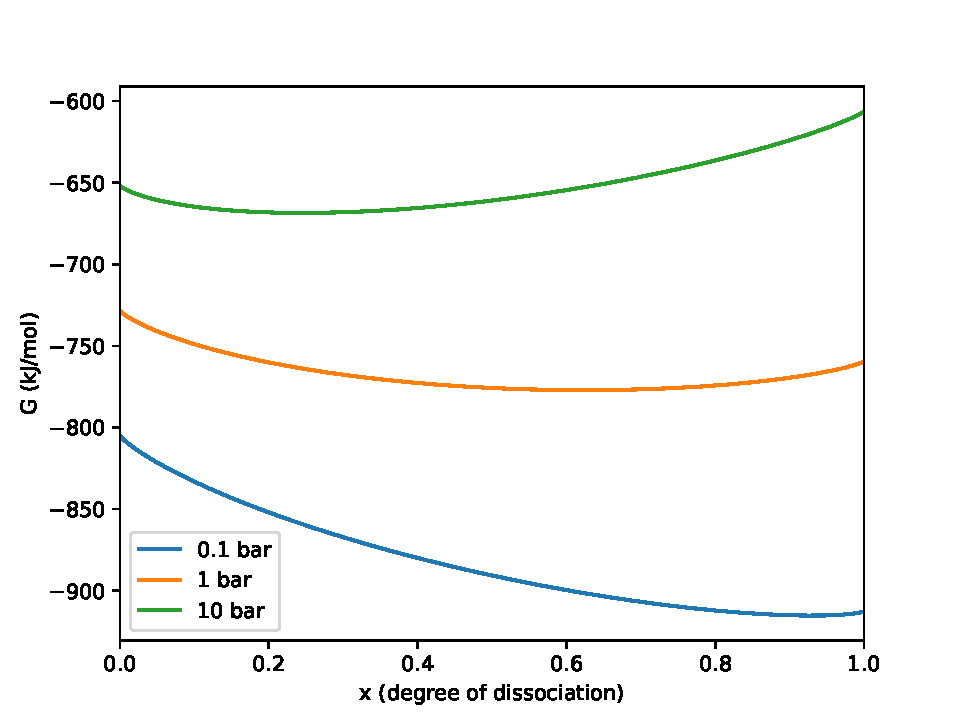
\includegraphics[width=0.7\textwidth]{assets/2 models/Gibbs.pdf}
            \caption{Gibbs free energy (G) plotted against the degree of dissociation (x) of hydrogen under three different pressures}
            \label{fig:Gibbs}
        \end{figure}

        A similar dissociation graph can be found with argon, but with three species. The Gibbs energy is then minimized to determine the molar fractions $y_i$ at which the mixture reaches equilibrium. From this, the enthalpy $H$ of the mixture was found. The $C_p$ of the mixture was then calculated from the enthalpy with:

        \begin{equation}
            C_p = \frac{\partial H}{\partial T}\bigg|_{p = const.}
        \end{equation}
        
        For argon, these calculated $C_p$ values were validated against values from CEA \cite{CEARUNRev4} in \autoref{fig:Cp_compare}.
        
        \begin{figure}[!ht]
            \centering
            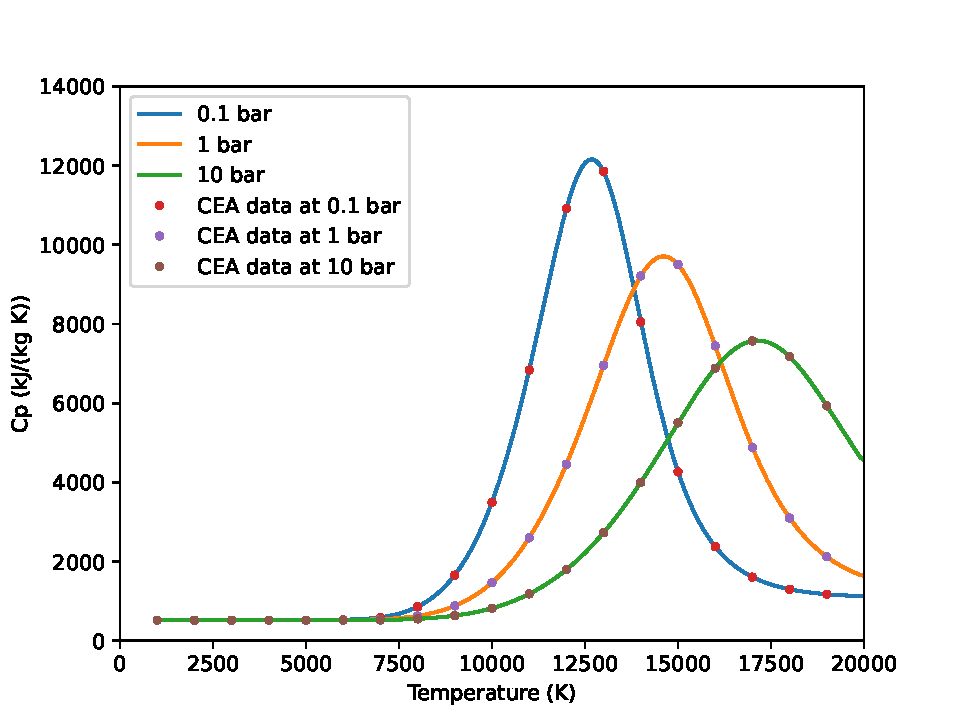
\includegraphics[width=0.7\textwidth]{assets/2 models/Cp_compare.pdf}
            \caption{Comparing calculated $C_p$ values of argon to those from CEA}
            \label{fig:Cp_compare}
        \end{figure}

        The properties of the argon plasma will be used as the basis of the 0D LSP model.
    
    \section{Bremsstrahlung}
        
        The main source of radiation found in LSP is Bremsstrahlung, or braking radiation. When an electron passes close to a heavier ion, it is deflected by the ion's electric field. This elastic collision releases a photon \todo{source}. The total radiated power of the collisions can then be calculated with the formulas presented in \autoref{tab:Brems_compare}.

        \begin{table}[!ht]
            \footnotesize
            \centering
            \caption{Comparison of Bremsstrahlung loss power}
            \label{tab:Brems_compare}
            \begin{tabularx}{\textwidth}{@{}lXX@{}}
            \toprule
            \textbf{Reference} & \textbf{Formula} & \textbf{SI Conversion} \\ \midrule
            \textcite{glasstoneControlledThermonuclearReactions1975}  & $P_\mathrm{br} = 1.57 \times 10^{-27} n_\mathrm{e} n_\mathrm{i} Z^2 T^{1/2}$ \: $\mathrm{ergs/(cm^3\cdot s)}$, with T in K. &   $P_\mathrm{br} = 1.57 \times 10^{-28} n_\mathrm{e} n_\mathrm{i} Z^2 T^{1/2} \: \mathrm{W/m^3}$  \\
            \textcite{rybickiRadiativeProcessesAstrophysics2004}      & $P_\mathrm{br} = 1.4 \times 10^{-27} n_\mathrm{e} n_\mathrm{i} Z^2 T^{1/2} \bar{g}_\mathrm{B}$ \: $\mathrm{ergs/(cm^3\cdot s)}$, with T in K.&  $P_\mathrm{br} = 1.68 \times 10^{-28} n_\mathrm{e} n_\mathrm{i} Z^2 T^{1/2} \: \mathrm{W/m^3}$, using $\bar{g}_\mathrm{B} (T)$ = 1.2\\
            \bottomrule          
            \end{tabularx}
        \end{table}

        The first relation, from \textcite{glasstoneControlledThermonuclearReactions1975} converted to SI, was used for the remainder of the calculations.

        There is also a question regarding whether the plasma is a surface emitter or a volume emitter. This is determined by calculating the plasma frequency at a typical electron density and comparing it to the wavelength of the light emitted by Bremsstrahlung. If the plasma frequency is higher than the wavelength of emitted Bremsstrahlung light, then it is cut off by the plasma; no light can escape the volume of the LSP cone, and it is a surface emitter. If it is lower, then the emitted photons are not blocked by the LSP and the cone is a volumetric emitter.
        
        The plasma frequency $\omega_\mathrm{p}$ is found with: 

        \begin{equation}
            \omega_\mathrm{p} = \sqrt{\frac{n_\mathrm{e} e^2}{\epsilon_\mathrm{0} m_\mathrm{e}}}
        \end{equation}

        With $n_\mathrm{e}$ the plasma electron density, $e$ the elementary charge, $\epsilon_\mathrm{0}$ the vacuum permittivity and $m_\mathrm{e}$ the electron mass.

        At \todo{todo} XX K and \todo{todo} XX Pa, an electron density of \todo{todo} XX is found. This results in $\omega_p =$ \qty{3.10e12}{Hz}. Considering visible light and above (> \qty{1e14}{Hz}) as the wavelengths of interest, the LSP is indeed a volume emitter.

    \section{Model setup}
        
        Finally, a simple 0D model was written in Python to attempt to explain the pressure rise seen in the LTP experiments. \autoref{fig:0D model} illustrates this model. Laser energy is focused into a volume of argon, creating an LSP cone. Energy is transferred from the LSP cone to the larger argon volume by Bremsstrahlung\todo{Have the arrow go from cone to volume, not outside!}. \todo{A part of the laser energy is also transmitted through the cone to the outside of the argon volume and lost.} The LSP is treated as an ideal gas.

        \begin{figure}[!ht]
            \centering
            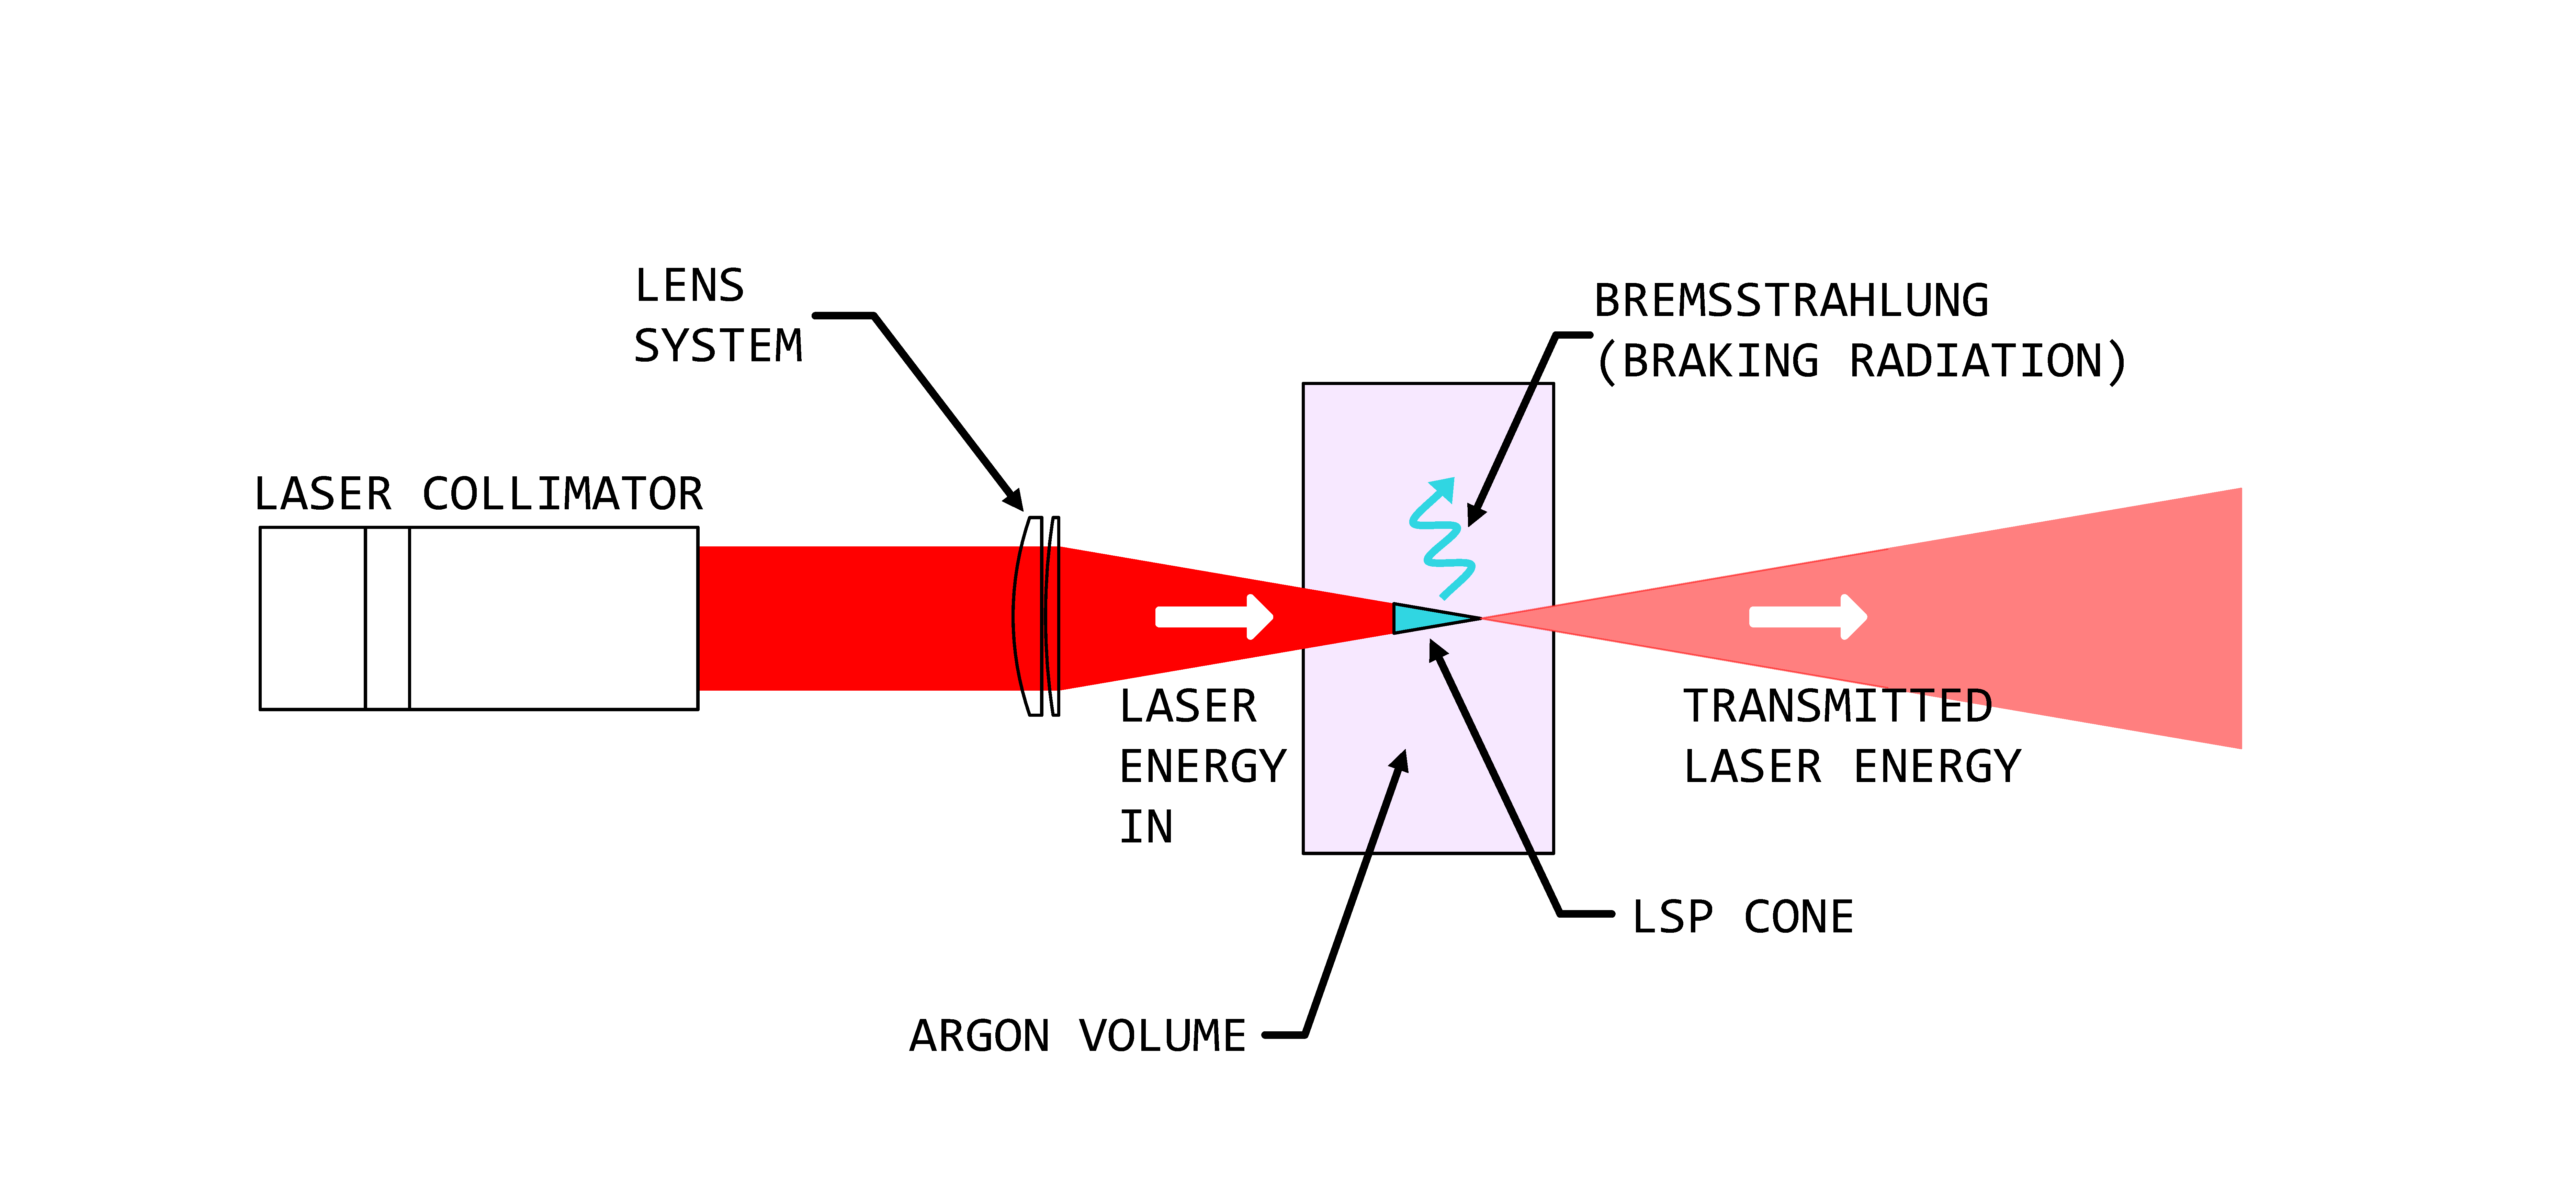
\includegraphics[width=0.85\textwidth]{assets/2 models/Modeling figure.pdf}
            \caption{0D model of an LSP inside a volume of pressurized argon}
            \label{fig:0D model}
        \end{figure}

        The calculation procedure that was implemented is as follows:

        \begin{enumerate}
            \item The volume and the mass of a cone of pure argon is found at the initial temperature (\qty{300}{K}) and pressure (\qty{20}{bar}). This mass will remain fixed for the rest of the problem
                \begin{equation}
                    huh
                \end{equation}
            \item Energy from the laser pulse is added to the cone at constant pressure and the new temperature at this step is found ($T_2$)
                \begin{equation}
                    E_\mathrm{plasma} = E_\mathrm{plasma} + P_\mathrm{laser} \times \mathrm{timestep} - P_\mathrm{loss} \times \mathrm{timestep}
                \end{equation}
                \begin{equation}
                    m_{plasma} (h_2 - h_1) = E_{laser}
                \end{equation}
                Where this equation is solved for 
            \item The number of moles in the LSP are found by minimizing the Gibbs free energy at the temperature and pressure of step 2. The new volume of the cone ($V_2$) is then found with the ideal gas law.
            \item The pressure increase in the chamber due to the isentropic expansion of the gas in the LSP cone is calculated ($p_4$)
                \begin{equation}
                    p_4 = p_\mathrm{ini} ((V_\mathrm{chamber} - V_\mathrm{plasma})/(V_\mathrm{chamber} - V_2))^k
                \end{equation}
            \item The radiated power from the LSP cone to the larger argon volume is determined using the Bremsstrahlung total power loss equation from \textcite{glasstoneControlledThermonuclearReactions1975}.
                \begin{equation}
                    P_\mathrm{br} = 1.57 \times 10^{-28} n_\mathrm{e} n_\mathrm{i} Z^2 T^{1/2}
                \end{equation}
            \item Steps 2 to 5 are looped until \qty{10}{ms}, when the laser shuts off. No more energy is added but Bremsstrahlung loss continues. The conservation of energy equation then becomes:
                \begin{equation}
                    E_\mathrm{plasma} = E_\mathrm{plasma} - P_\mathrm{loss} \times \mathrm{timestep}
                \end{equation}
        \end{enumerate}
        
        To determine an upper bound on power loss, a switch was implemented to change Bremsstrahlung loss to blackbody radiation loss.

    \section{Model results}

        \begin{figure}[!ht]
            \centering
            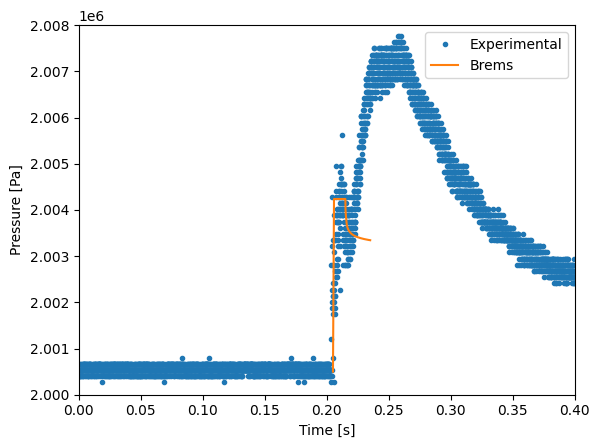
\includegraphics[width=0.85\textwidth]{assets/2 models/Brems vs exp graph.png}
            \caption{Experimental data compared to the 0D model, with both Bremsstrahlung and blackbody losses}
            \label{fig:Model results}
        \end{figure}

        \todo{Add blackbody radiation loss, add laser pulse "on" area.} From these iterations, \autoref{fig:Model results} was drawn. Using Bremsstrahlung loss, the model appropriately approximates the first peak seen in the experimental data. Once the gas cools down enough and stops being ionized, Bremsstrahlung loss stops. The LSP cone in the model is then stable at approximately a temperature of \qty{5200}{K} and a pressure of \qty{2.003}{MPa}. The second peak could be explained by the fact that the energy in the cone is then communicated to the rest of the argon volume, equalizing temperatures and pressures.